\subsection{Performance}
\label{sec:Performance}

\NOTE{\emph{Length:} 1 p., \emph{Responsible:} Tony}

\NOTE{Debatable whether and to what extent this should be included. Maybe only partial results could be presented here.}

Besides the size of the transformation specifications and their correctness, the performance of the respective solutions for different model sizes is an interesting question. To this end, scalability tests for each tool and each transformation direction were performed both in batch as well in an incremental mode of operation. The tests have been performed on the same machine and each tool was tested separately to avoid side effects due to memory leaks or other implementation issues in the respective solutions. 

The performance was measured on a machine with Intel Core i7-4770 CPU, running at 3.40 GHz, 16 GB of DDR3 RAM and Windows 10 64-bit OS. Java 1.8.0\_191 was used as well Eclipse Neon (4.6.3) with EMF version 2.12.0.

For the test scenarios, random models are created and transformed. In a loop, the model size is increased in each step until the threshold of model elements is reached. 

To cope with measurement inconsistencies, each test is carried out three times for the same model size and the median of the measured times is computed. 

While the batch tests (in both forward and backward direction) require to transform constantly growing models, the incremental tests only measure the time that a single edit operation needs (after the initial model state has been established by the tool). For all test runs, we set a threshold of 10 minutes. I.e. if an execution of a transformation for a certain model size requires more than 600s, we stop the test for that tool. Nevertheless performance testing all six solution took more than two weeks.

Please note that in the following two figures are given for each scalability test. In all figures the x-axis denotes the number of elements in the respective models while the y-axis denotes the required time for the model transformation in seconds. The first figure presents the results with both axes scaled in a linear way while in the second figure a logarithmic scale is used for both the x and the y axis. Using a logarithmic scale, tools with poor scalability have less influence on the readability of the diagram. Furthermore, the difference among the tools becomes more evident even for smaller model sizes.
Please note that is was not possible to measure times for the EVL+Strace solution, since it does not implement the benchmarx infrastructure. In addition, there is no test suite available which allows to execute all tests for EVL+Strace automatically. Furthermore, the JTL solution fails with errors for even very small model sizes (approx. 6000 elements). As a consequence it was only possible to determine exeuction times for JTL with models up to 5502 elements. But nevertheless it is fair to say that JTL does not scale at all in our tests.


\begin{figure}[h!]
	\centering
	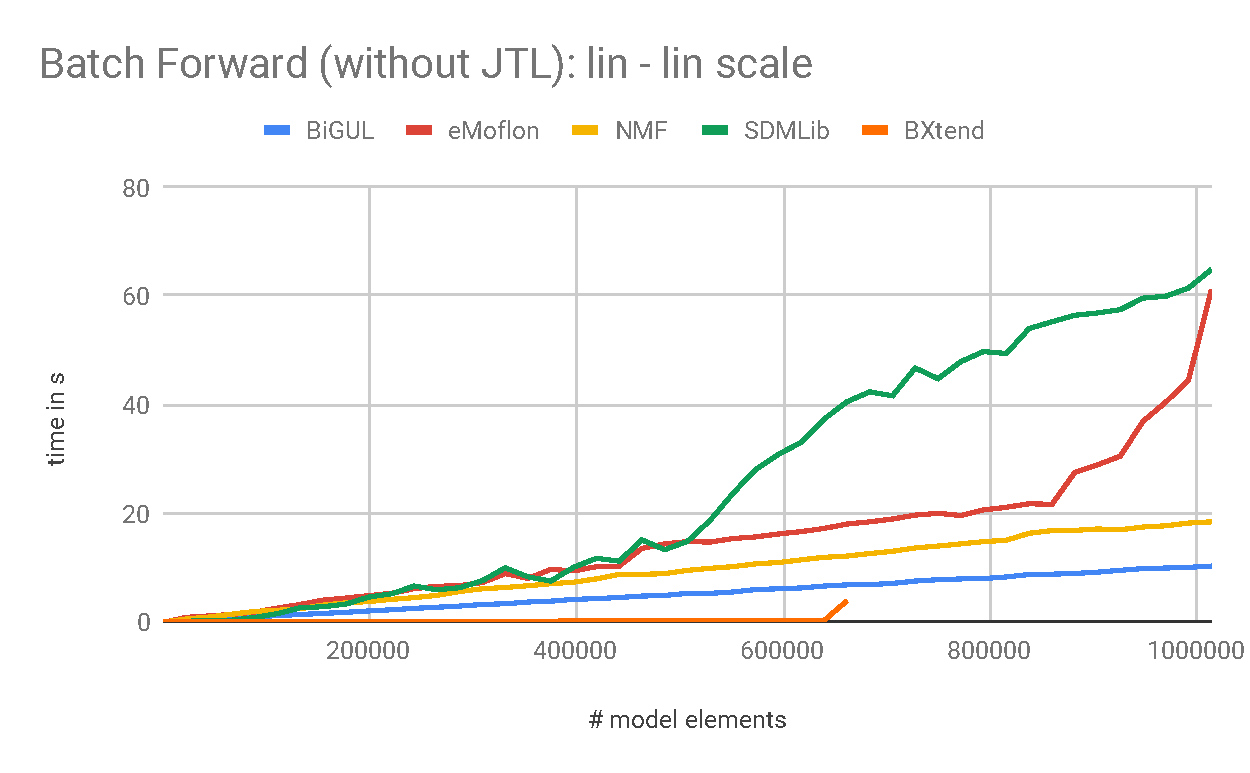
\includegraphics[width=\columnwidth]{diagrams/scalability/BFlinlin}
	\caption{Batch Forward (without JTL), both axis in linear scale.}
	\label{fig:scalabilityBatchFWDlin}
\end{figure}

Figure \ref{fig:scalabilityBatchFWDlin} depicts the obtained results for the batch forward transformation using a linear scale of both axes. Graphs for all tools except JTL are presented. While all tools only show a moderate growth in computation time for increasing model sizes, JVM-based tools like SDMLib, eMoflon and BXtend show significant increases at a certain model size. This behavior results from memory management in Java. Furthermore, BXtend fails with a garbage collector exception and does not reach the maximum model size used in our test runs. 

\begin{figure}[h!]
	\centering
	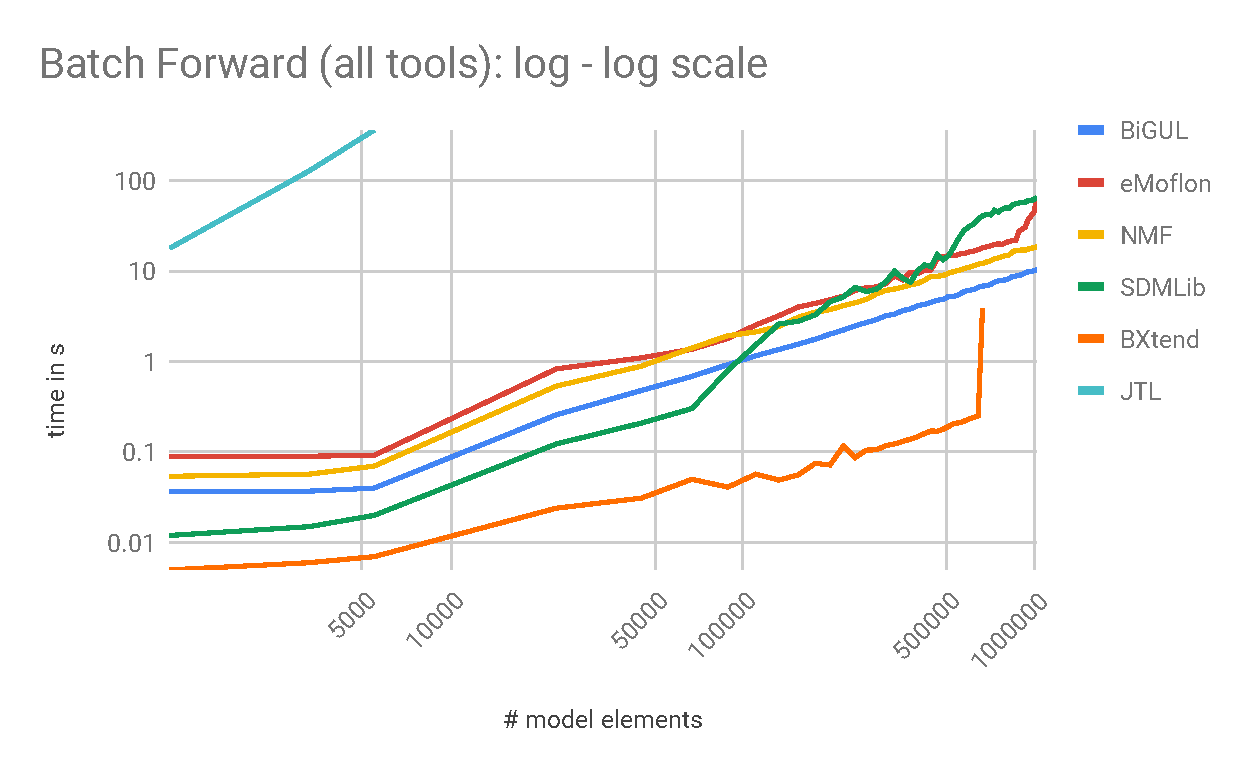
\includegraphics[width=\columnwidth]{diagrams/scalability/BFloglog}
	\caption{Batch Forward (all tools), both axis in logarithmic scale.}
	\label{fig:scalabilityBatchFWDlog}
\end{figure}

Figure \ref{fig:scalabilityBatchFWDlog} depicts the results for the same transformation, but now both axes use a logarithmic scale. It is obvious that JTL fails for models with more than 5500 elements. And even for models with less than 5500 elements, a significantly greater computation time is required in comparison to the other solutions even for models with 1.000.000 elements. This Figure also shows that BXtend is the fastest solution for the batch forward transformation, until the Java memory problems stopped the test. The different graphs show that BiGUL, eMoflon, NMF, SDMLib and BXtend scale in a linear way until a certain size of the model is reached. After that point a moderate polynomial growth in computation time may be observed.


\begin{figure}[h!]
	\centering
	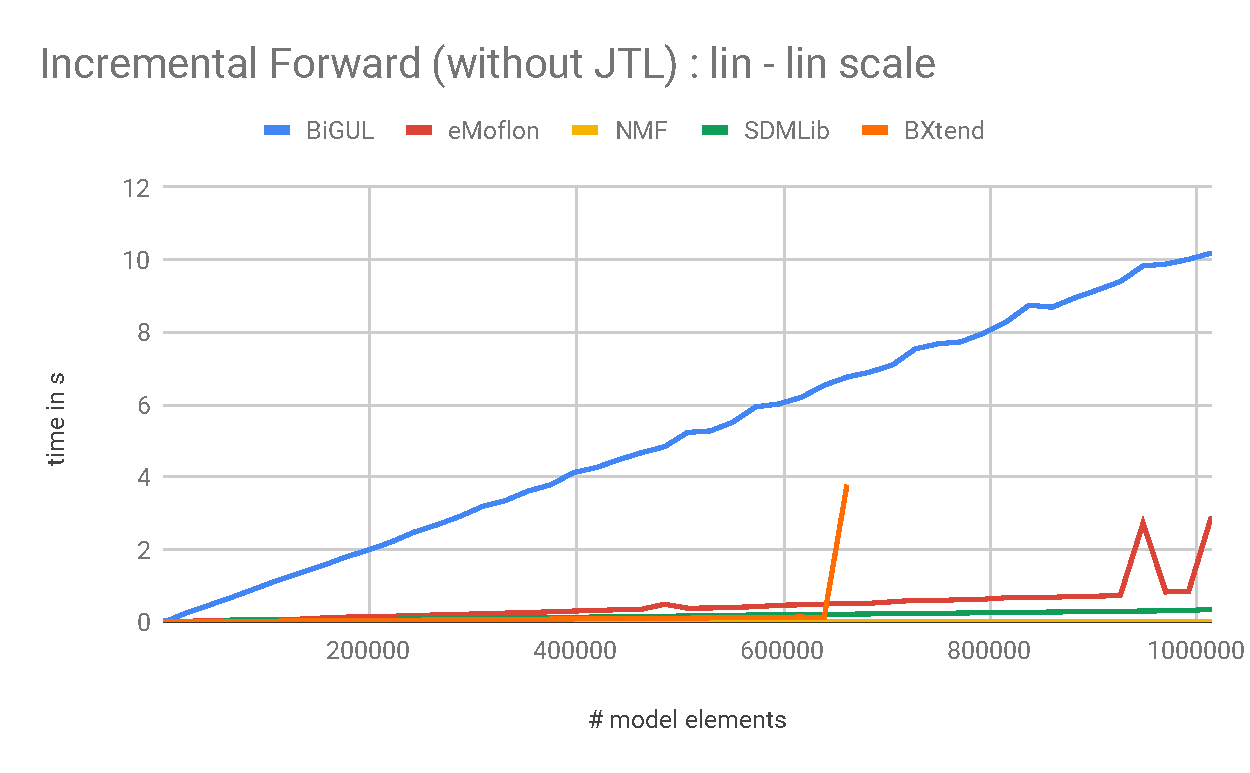
\includegraphics[width=\columnwidth]{diagrams/scalability/IFlinlin}
	\caption{Incremental Forward (without JTL), both axis in linear scale.}
	\label{fig:scalabilityIncrFWDlin}
\end{figure}

The observations for the incremental forward transformations reveal that BiGUL does not operate in an incremental way. It requires the same amount of computation time as for the batch forward case, while all other tool (except JTL) perform the incremental transformation very efficiently. Figure \ref{fig:scalabilityIncrFWDlin} depicts the graphs for the obtained computation times with both axes scaled in a linear way.

\begin{figure}[h!]
	\centering
	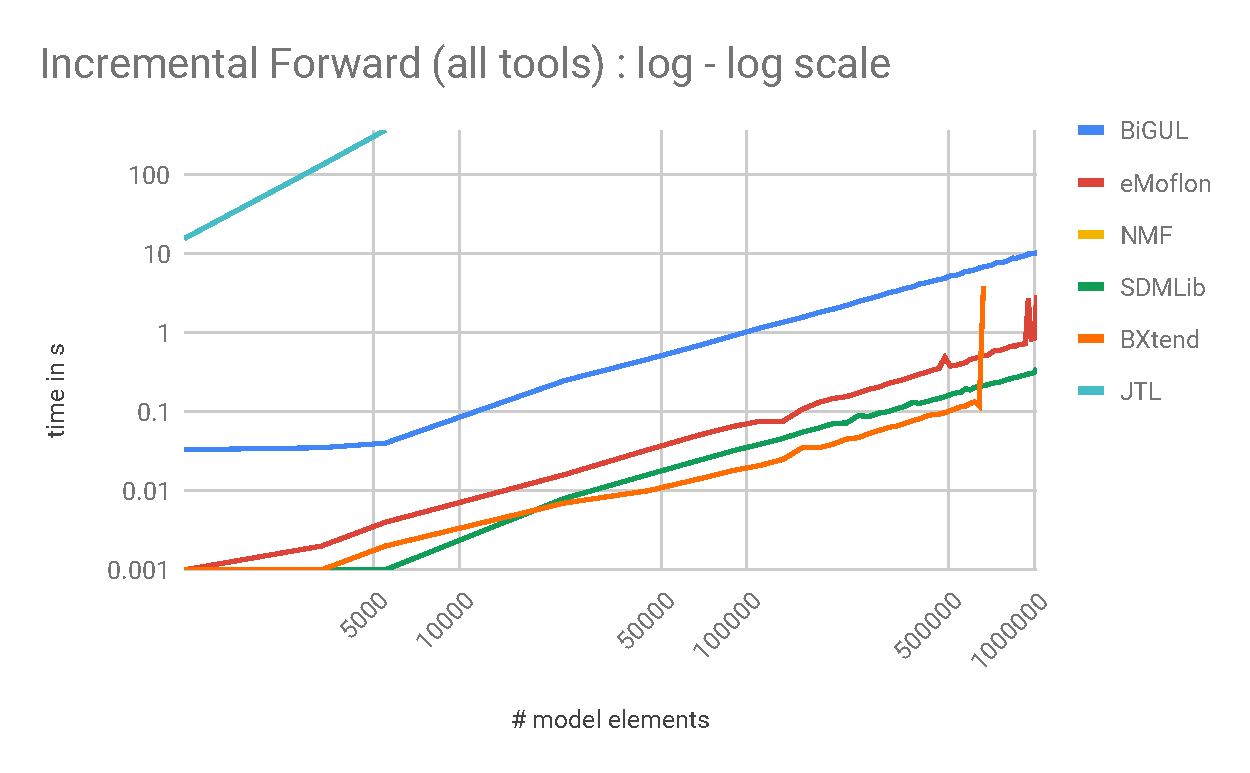
\includegraphics[width=\columnwidth]{diagrams/scalability/IFloglog}
	\caption{Incremental Forward (all tools), both axis in logarithmic scale.}
	\label{fig:scalabilityIncrFWDlog}
\end{figure}

In contrast, Figure \ref{fig:scalabilityIncrFWDlog} shows the same results with logarithmic scale and with the results for JTL. Again it is evident that JTL has at least polynomial complexity. All other solutions scale much better with increasing model sizes. 

\begin{figure}[h!]
	\centering
	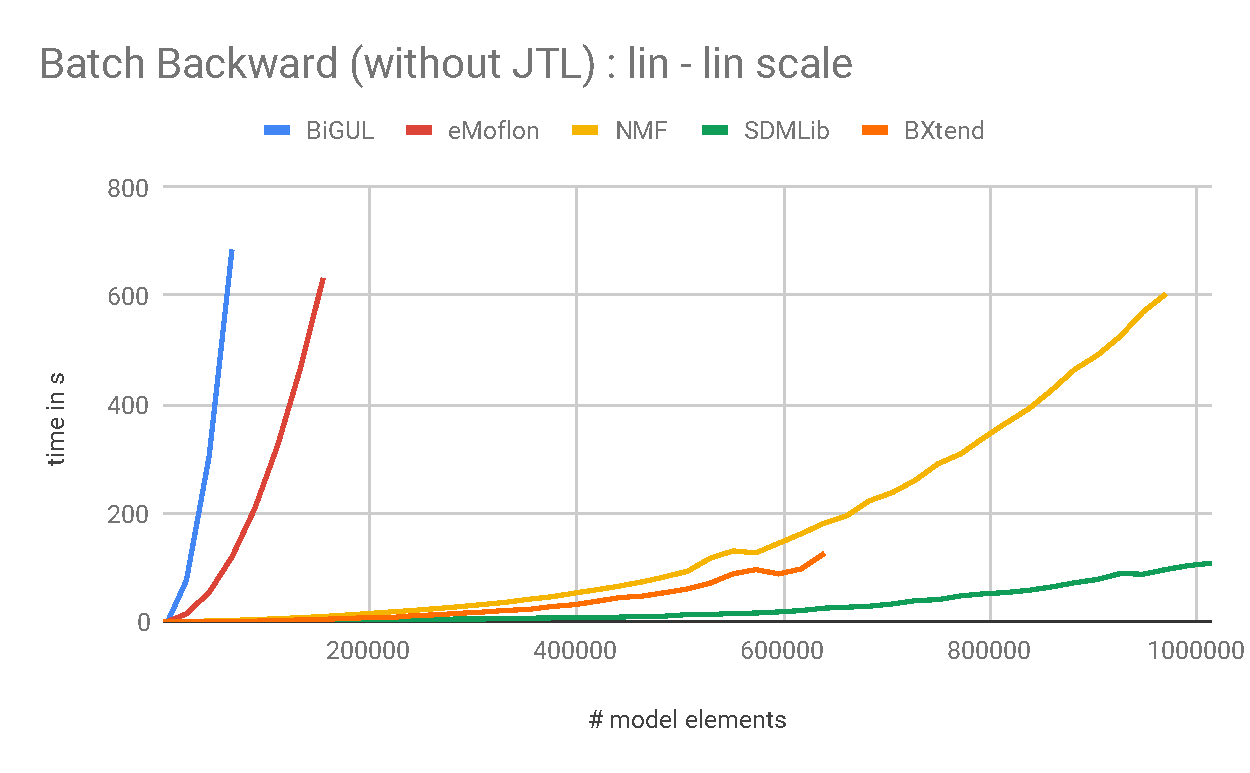
\includegraphics[width=\columnwidth]{diagrams/scalability/BBlinlin}
	\caption{Batch Backward (without JTL), both axis in linear scale.}
	\label{fig:scalabilityBatchBWDlin}
\end{figure}

Graphs for the batch backward transformations for all tools except JTL are presented in Figure \ref{fig:scalabilityBatchBWDlin}. Again, a linear scale on both axes is used. The obtained numbers indicate that the backward transformation requires significantly more computation time as the forward case for all tools. Probably this is due the configuration options. Furthermore, BiGUL and eMoflon scale bad compared to the other solutions and reach the time limit for models with 67.000 (BiGUL) and 155.000 (eMoflon) elements. 
\NOTE{Tony, please add your explanation for the bad results for eMolon here}
The only solution that reached the maximum model size within the time limit was SDMLib. NMF reaches the 600 second limit at a model size of approx. 960.000 elements. Again the BXtend solution fails with a Java garbage collector exception at a model size of approx. 670.000 elements.

\begin{figure}[h!]
	\centering
	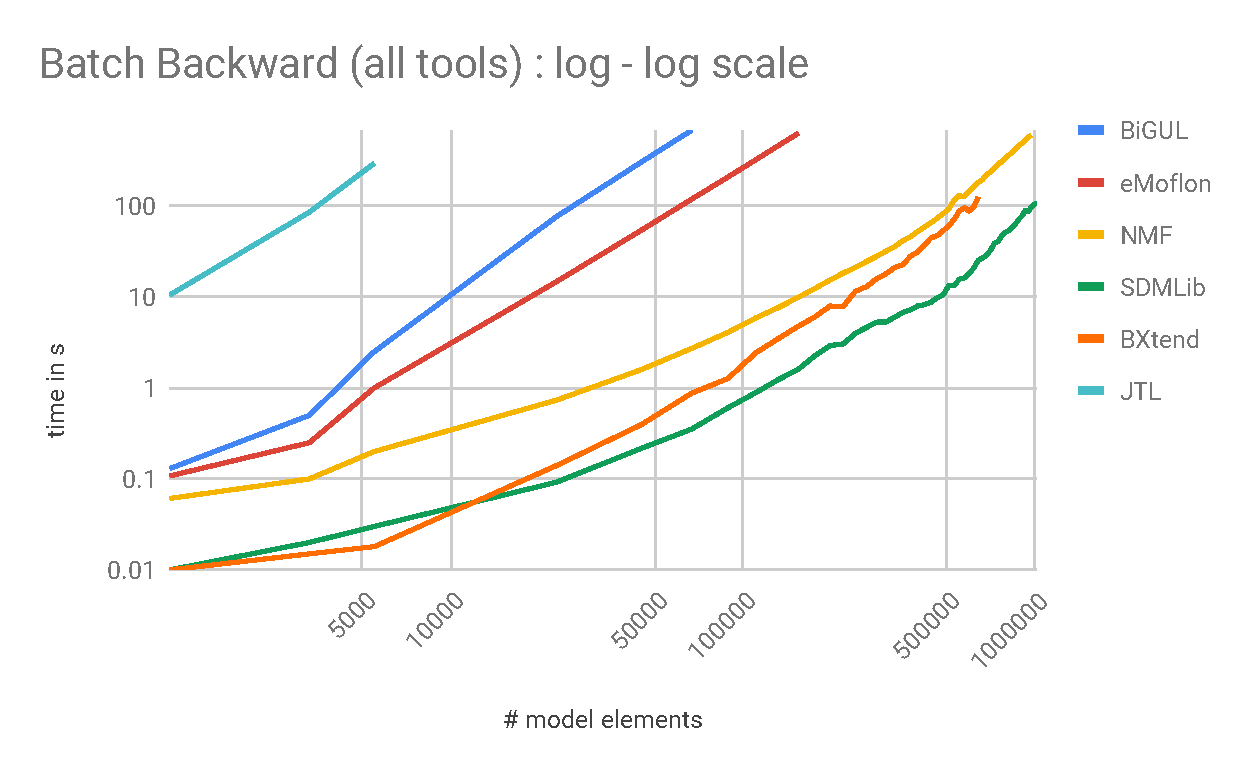
\includegraphics[width=\columnwidth]{diagrams/scalability/BBloglog}
	\caption{Batch Backward (all tools), both axis in logarithmic scale.}
	\label{fig:scalabilityBatchBWDlog}
\end{figure}

The same results shown in a diagram with logarithmic scale on both axes (c.f., Figure \ref{fig:scalabilityBatchBWDlog}) reveal small differences in computation times of NMF, BXtend and SDMLib, while BiGUL and eMoflon scale worse. JTL again does not scale at all.

\begin{figure}[h!]
	\centering
	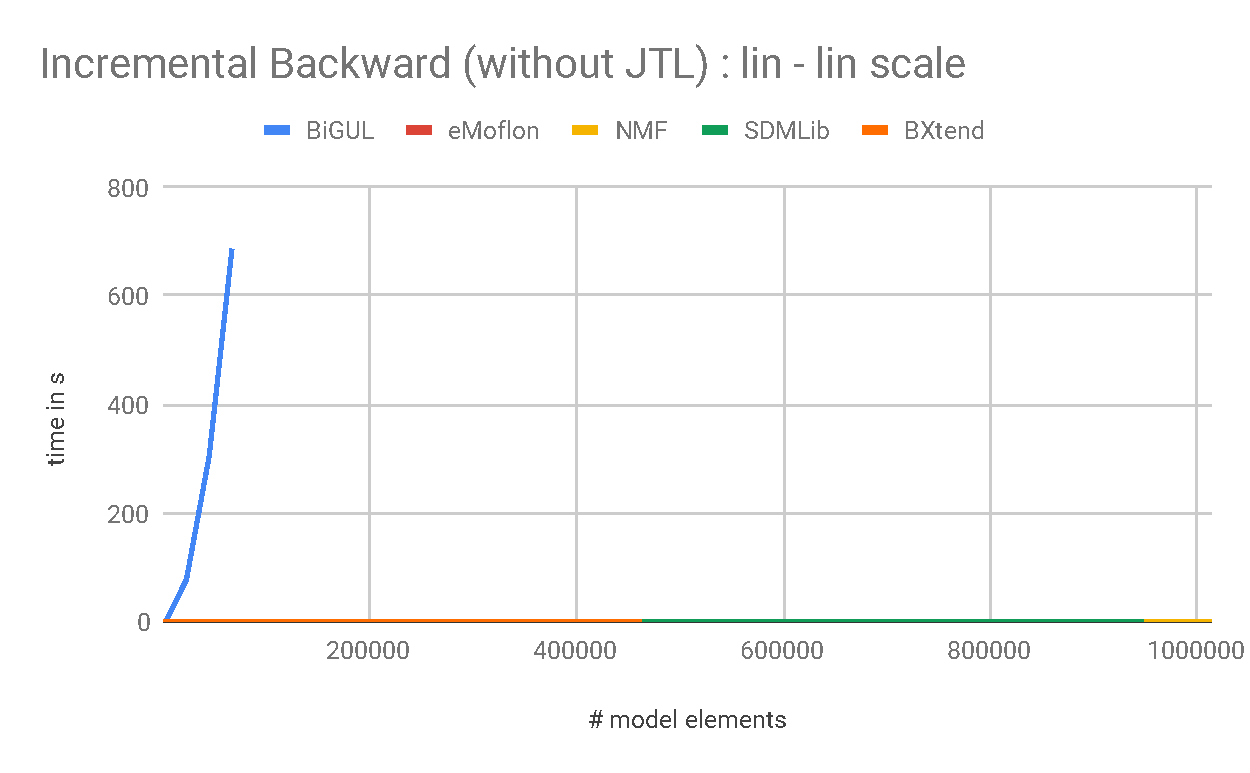
\includegraphics[width=\columnwidth]{diagrams/scalability/IBlinlin}
	\caption{Incremental Backward (without JTL), both axis in linear scale.}
	\label{fig:scalabilityIncrBWDlin}
\end{figure}

The last test was an incremental backward transformation. The incremental operation was an atomic edit step which had to be recognized in a constantly growing model. Results are shown in Figure \ref{fig:scalabilityIncrBWDlin}, with both axes scaled in a linear way. Since BiGUL does not work in an incremental mode of operation, the times are the same as for the batch transformation, while all other tools in this diagram (again JTL was omitted here) show a much better performance.

\begin{figure}[h!]
	\centering
	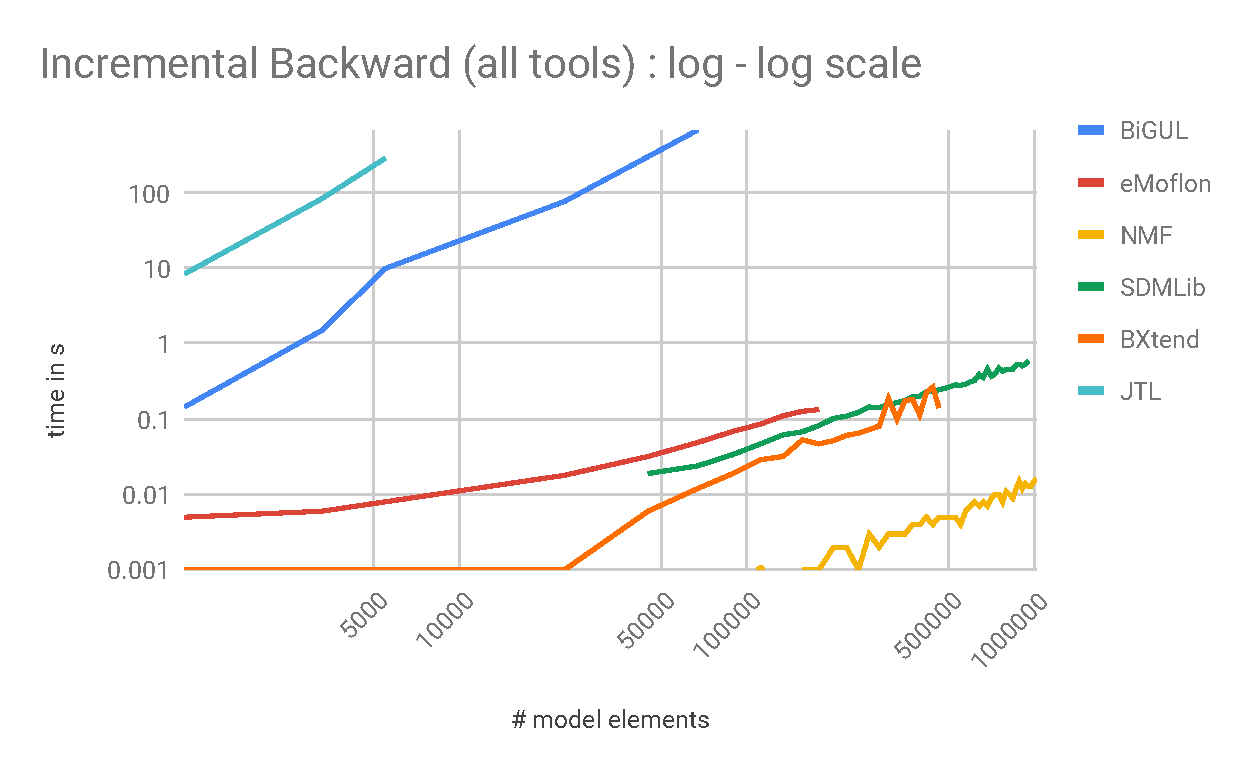
\includegraphics[width=\columnwidth]{diagrams/scalability/IBloglog}
	\caption{Incremental Backward (all tools), both axis in logarithmic scale.}
	\label{fig:scalabilityIncrBWDlog}
\end{figure}

The differences among the tools become clearer in the diagram using logarithmic scale, as shown in Figure \ref{fig:scalabilityIncrBWDlog}. NMF shows the best performance, even in very large models. BXtend also performs very good until the memory problems occur, as well as eMoflon and SDMLib.